\chapter{Revisão da Literatura}


\section{Fundamentação Teórica}

Esta seção reúne conceitos e autores do livro \cite{DantzigThapa:1997} e que fundamentam a modelagem proposta neste trabalho. São discutidos os princípios da Programação Linear, a estrutura do Problema de Transporte e sua interpretação como um problema de fluxo, bem como a extensão para Programação Linear Inteira, necessária para representar adequadamente o problema de distribuição de vacinas.

\subsection{Programação Linear}

A Programação Linear (PL) é uma técnica de otimização utilizada para modelar problemas em que se deseja minimizar ou maximizar uma função objetivo linear sujeita a um conjunto de restrições também lineares.

De forma geral, um problema de Programação Linear pode ser expresso como:

\[
\min \; z = c^T x \quad \text{sujeito a} \quad Ax \le b, \; x \in \mathbb{R}_{\geq 0}
\]

onde:
\begin{itemize}
    \item $x$ representa o vetor de variáveis de decisão;
    \item $c$ representa os coeficientes da função objetivo;
    \item $A$ representa a matriz de coeficientes das restrições;
    \item $b$ representa os limites das restrições.
\end{itemize}

A principal característica desse tipo de modelo é a linearidade, que implica que tanto a função objetivo quanto as restrições representam relações proporcionais entre as variáveis.

No contexto logístico, a Programação Linear é amplamente utilizada para modelar problemas de alocação de recursos, transporte e distribuição, pois permite representar decisões de envio de produtos entre diferentes pontos de uma rede.

\subsection{Problema de Transporte}

O Problema de Transporte é um caso particular da Programação Linear que modela a distribuição de um produto a partir de múltiplas origens para múltiplos destinos.

Considere:
\begin{itemize}
    \item um conjunto de origens $i \in I$, cada uma com uma quantidade disponível $s_i$;
    \item um conjunto de destinos $j \in J$, cada um com uma demanda $d_j$;
    \item um custo de transporte $c_{ij}$ associado ao envio de uma unidade do produto da origem $i$ para o destino $j$.
\end{itemize}

Define-se a variável de decisão:

\[
x_{ij} \geq 0
\]

onde $x_{ij}$ representa a quantidade transportada da origem $i$ para o destino $j$.

O modelo clássico é dado por:

\[
\min \sum_{i \in I} \sum_{j \in J} c_{ij} x_{ij}
\]

sujeito a:

\[
\sum_{j \in J} x_{ij} = a_i, \quad \forall i \in I
\]

\[
\sum_{i \in I} x_{ij} = b_j, \quad \forall j \in J
\]

\[
x_{ij} \geq 0
\]

A primeira restrição garante que toda a oferta disponível em cada origem seja distribuída, enquanto a segunda garante que toda a demanda dos destinos seja atendida.

\begin{figure}[ht]
    \centering
    \caption{Esquema de Rede para o Problema de Transporte}
    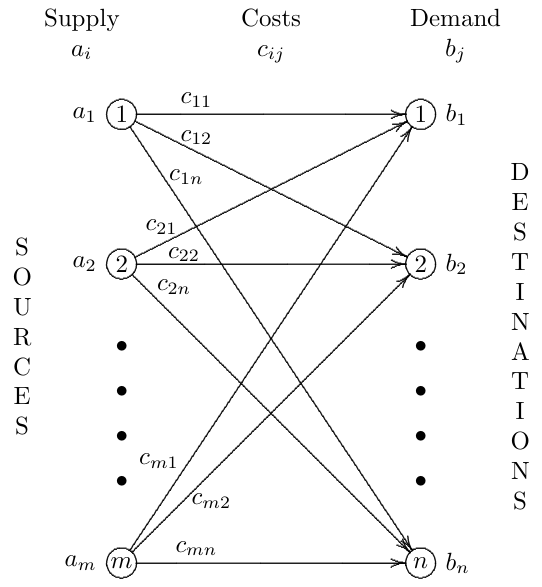
\includegraphics[width=10cm]{figuras/transportation_problem.png} 
    \legend{Fonte: Dantzig e Thapa (1997, p. 207)}
    \label{fig:network_dantzig}
\end{figure}

\subsection{Interpretação como Problema de Fluxo}

O Problema de Transporte pode ser interpretado como um problema de fluxo em rede.

Nessa interpretação:
\begin{itemize}
    \item cada origem é um nó com oferta;
    \item cada destino é um nó com demanda;
    \item cada par $(i,j)$ representa uma aresta pela qual o fluxo pode ocorrer.
\end{itemize}

A variável $x_{ij}$ representa o fluxo que percorre a aresta que liga $i$ a $j$.

Uma propriedade fundamental desse tipo de modelo é a \textbf{conservação de fluxo}. Isso significa que:
\begin{itemize}
    \item todo o fluxo que sai das origens deve chegar aos destinos;
    \item não há criação ou perda de fluxo ao longo da rede.
\end{itemize}

Essa propriedade é diretamente refletida nas restrições do modelo, que impõem equilíbrio entre oferta e demanda.

\subsection{Balanceamento do Problema}

No modelo clássico do Problema de Transporte, assume-se que a oferta total é igual à demanda total, ou seja:

\[
\sum_{i \in I} a_i = \sum_{j \in J} b_j
\]

No entanto, essa hipótese não é adotada neste trabalho.

Na modelagem proposta, permite-se que a quantidade total ofertada seja superior à quantidade demandada, refletindo situações reais em que nem todas as vacinas disponíveis precisam ser redistribuídas, ou seja:

\[
\sum_{i \in I} a_i \ge \sum_{j \in J} d_j
\]

Para isso, a restrição de oferta é modelada como uma desigualdade, permitindo que parte do estoque permaneça no município de origem, enquanto a restrição de demanda é mantida como igualdade, garantindo o atendimento integral das necessidades dos municípios de destino.

Essa abordagem torna o modelo mais aderente à realidade operacional do sistema de distribuição de vacinas.

\subsection{Limitações do Modelo Clássico}

Apesar de sua utilidade, o Problema de Transporte clássico apresenta limitações importantes quando aplicado a problemas reais.

Uma das principais limitações é a hipótese de divisibilidade das variáveis. No modelo linear contínuo, as variáveis $x_{ij}$ podem assumir valores fracionários.

No contexto da distribuição de vacinas, essa hipótese não é adequada, pois:
\begin{itemize}
    \item as variáveis representam quantidades físicas de doses;
    \item não é possível transportar frações de doses;
    \item as decisões logísticas envolvem unidades discretas.
\end{itemize}

Além disso, problemas reais frequentemente incluem:
\begin{itemize}
    \item múltiplos tipos de produtos;
    \item restrições adicionais de capacidade;
    \item limitações operacionais;
    \item critérios de prioridade.
\end{itemize}

Esses aspectos não são completamente capturados pelo modelo clássico.

\subsection{Programação Linear Inteira}

Para representar adequadamente decisões discretas, utiliza-se a Programação Linear Inteira (PLI).

Um problema de Programação Linear Inteira pode ser expresso como:

\[
\min \; z = c^T x \quad \text{sujeito a} \quad Ax \le b, \; x \in \mathbb{Z}_{\geq 0}
\]

A principal diferença em relação à Programação Linear está na restrição de integralidade, que impõe que as variáveis de decisão assumam apenas valores inteiros.

Essa restrição altera significativamente a natureza do problema:
\begin{itemize}
    \item o conjunto de soluções possíveis deixa de ser contínuo;
    \item a busca pela solução ótima ocorre em um espaço discreto;
    \item o problema se torna mais complexo do ponto de vista computacional.
\end{itemize}

\subsection{Relação com o Problema Proposto}

O problema de distribuição de vacinas estudado neste trabalho pode ser interpretado como uma extensão do Problema de Transporte clássico.

As principais diferenças incluem:

\begin{itemize}
    \item presença de múltiplos tipos de vacinas;
    \item inclusão de restrições de capacidade de transporte;
    \item consideração de critérios temporais relacionados à validade;
    \item necessidade de variáveis inteiras;
    \item possibilidade de múltiplas etapas logísticas.
\end{itemize}

Dessa forma, o modelo proposto se enquadra como um Problema de Programação Linear Inteira aplicado a redes de transporte, no qual a estrutura clássica é estendida para capturar características operacionais mais realistas.